% Operations schematic for the German student initiative "Studenten bilden Schüler e.V."
% See https://studenten-bilden-schueler.de.

\documentclass[tikz,svgnames]{standalone}

\usepackage[utf8]{inputenc}
\usepackage[T1]{fontenc}

\usetikzlibrary{positioning,decorations.text}

\renewcommand{\familydefault}{\sfdefault}

\tikzset{
    entity/.style={fill=#1!70,text=white,rounded corners,inner sep=1ex,font=\bfseries},
    action/.style={->,thick,postaction={decorate,decoration={raise=2pt,text along path,text align=center,text={|\scriptsize|#1}}}},
    non-ovs action/.style={->,DarkGray,postaction={decorate,decoration={raise=2pt,text along path,text align=center,text={|\scriptsize\color{DarkGray}|#1}}}},
    action/.default=
}

\begin{document}
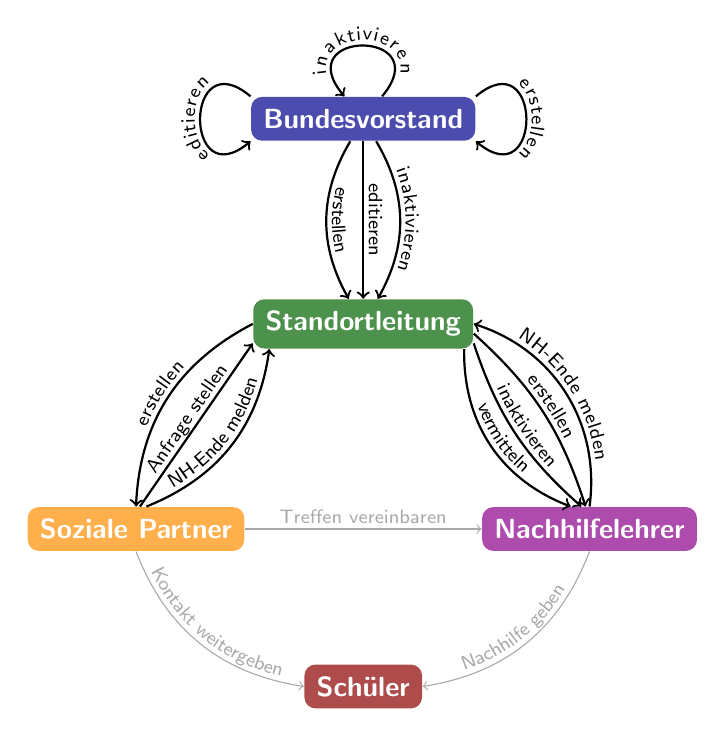
\begin{tikzpicture}[node distance=2 and 0.1]

  % Entities
  \node[entity=DarkBlue] (BV) {Bundesvorstand};

  \node[entity=DarkGreen,below=of BV] (SL) {Standortleitung};

  \node[entity=DarkOrange,below left=of SL] (SP) {Soziale Partner};

  \node[entity=DarkMagenta,below right=of SL] (NHL) {Nachhilfelehrer};

  \node[entity=DarkRed,below=4 of SL] (SC) {Schüler};

  % Actions
  % BV to BV
  \draw[action=erstellen] (BV.north east) to [in=-40,out=40,looseness=5] (BV.south east);
  \draw[action=editieren,decoration=reverse path] (BV.north west) to [in=220,out=140,looseness=5] (BV.south west);
  \draw[action=inaktivieren,decoration=reverse path] (BV.50) to [in=130,out=50,looseness=6] (BV.130);

  % BV to SL
  \draw[action=erstellen] (BV) to [bend right] (SL);
  \draw[action=editieren] (BV) to (SL);
  \draw[action=inaktivieren] (BV) to [bend left] (SL);

  % SL to SP
  \draw[action=erstellen,decoration=reverse path] (SL.west) to [bend right] (SP.north);


  % SP to SL
  \draw[action=Anfrage stellen] (SP.80) to (SL.190);
  \draw[action=NH-Ende melden] (SP.65) to [bend right] (SL.195);

  % SL to NHL
  \draw[action=inaktivieren] (SL.-10) to [bend right=15] (NHL.110);
  \draw[action=vermitteln] (SL.-14) to [bend right=35] (NHL.130);
  \draw[action=erstellen] (SL.-5) to [bend left=15] (NHL.100);

  % NHL to SL
  \draw[action=NH-Ende melden,decoration=reverse path] (NHL.north) to [bend right=40] (SL.east);

  % SP to SC
  \draw[non-ovs action=Kontakt weitergeben] (SP.south) to [bend right] (SC.west);

  % SP to NHL
  \draw[non-ovs action=Treffen vereinbaren] (SP.east) to (NHL.west);

  % NHL to SC
  \draw[non-ovs action=Nachhilfe geben,decoration=reverse path] (NHL.south) to [bend left] (SC.east);
\end{tikzpicture}
\end{document}